\chapter{Web of Things}
\label{web-of-things}

\section{Web of Things vs Internet of Things}

\textbf{Internet of Things: una definizione} \\

Internet of Things è un sistema di oggetti fisici che possono essere
rilevati, monitorati, controllati o con cui si può interagire con
devices elettronici, che comunicano fra loro attraverso interfacce di rete
e, infine, che possono collegarsi a Internet.

C'è una nuova classe di oggetti che sta per entrare nelle nostre case:
le \textbf{Smart Things}. Una Smart Thing è un oggetto fisico ``digitalmente
aumentato'' con una o più delle seguenti caratteristiche:

\begin{itemize}
  \item Sensori (temperatura, luce, movimento, ecc.)
  \item Attuatori (displays, suoni, etc.)
  \item Proprietà computazionali (possono eseguire programmi)
  \item Interfacce di comunicazione (wired or wireless)
\end{itemize}

\begin{figure}[H]
  \centering
  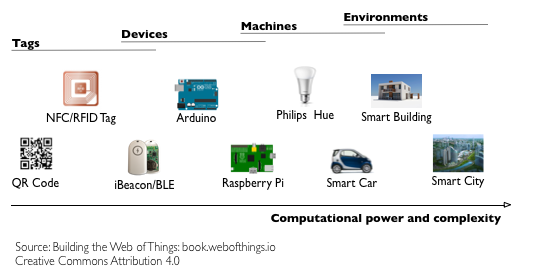
\includegraphics[scale=0.6]{iotland.png}
  \caption{Scenario IoT. IoT è una rete di oggetti collegati ad Internet.}
  \label{fig:iotland}
\end{figure}

Il nome ``Internet of Things'' significa semplicemente che un oggetto (e i
suoi servizi o dati da/verso esso) può essere acceduto e processato da altre
applicazioni attraverso l'esistente infrastruttura di Internet.

Le limitazioni dell'IoT diventano evidenti non appena si vuole integrare
dispositivi di vari produttori in una singola applicazione o sistema.

\begin{figure}[H]
  \centering
  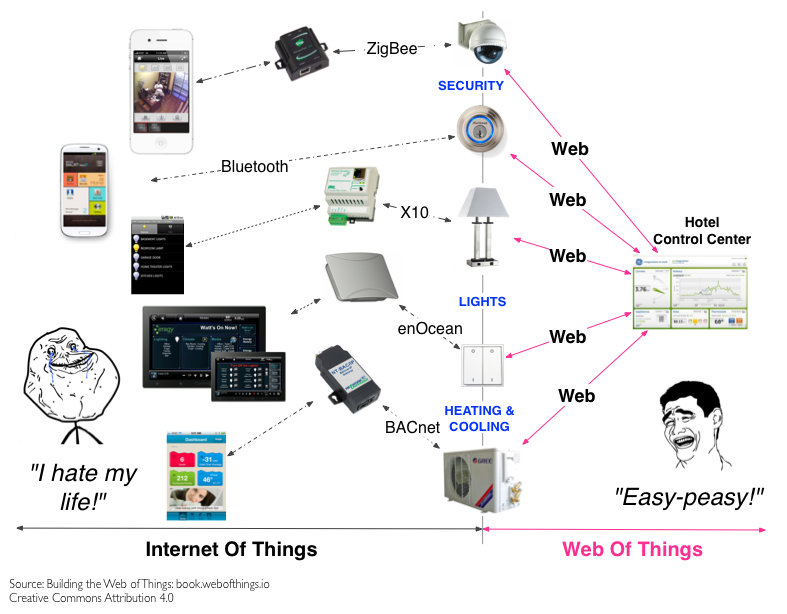
\includegraphics[scale=0.5]{integration_problem.png}
  \caption{Nell'IoT, oggi esistono centinaia di protocolli incompatibili.
Ciò rende l'integrazione di dati e servizi da vari dispositivi estremamente
complessa e costosa.}
  \label{fig:integration_problem}
\end{figure}

\subsection{Sfuggire al pattern ``un device, un protocollo, una sola app''}

Nel Web of Things (non IoT!), è possibile accedere a qualsiasi dispositivo
utilizzando protocolli web standard.

Collegare dispositivi eterogenei al Web rende la loro integrazione in sistemi
più ampi e/o applicazioni molto più semplice.

L'idea di applicare gli strumenti e le tecniche presenti nel
Web allo sviluppo di scenari IoT si chiama Web of Things.

Mentre IoT si occupa di risolvere problemi di rete, il Web of Things si basa
esclusivamente su protocolli e strumenti a livello di applicazione.

Mappare un qualsiasi dispositivo in un contesto Web rende agnostico il
Web of Things rispetto ai protocolli di livello fisico e di trasporto
utilizzati dai dispositivi.

\begin{figure}[H]
  \centering
  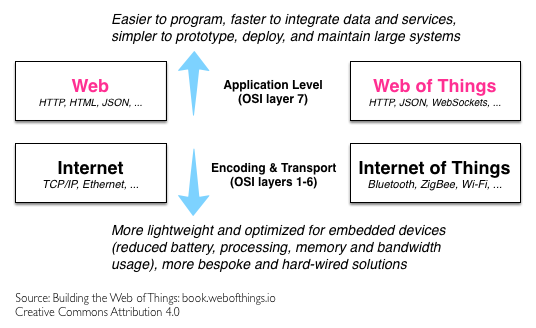
\includegraphics[scale=0.6]{iotstack.png}
  \caption{Il Web of Things riguarda solo il più alto livello OSI, che
gestisce applicazioni, servizi e dati.
Lavorare con un elevato livello di astrazione consente di collegare dati
e servizi da molti dispositivi indipendentemente dai veri e propri protocolli
di trasporto usati.
Al contrario, l'Internet of Things non sostiene un particolare protocollo a
livello di applicazione e di solito si concentra sugli strati inferiori dello
Stack OSI.}
  \label{fig:iotstack}
\end{figure}

\textbf{Lo scopo è quello di accedere agli oggetti in modo standardizzato e
trasparente.}

\begin{figure}[H]
  \centering
  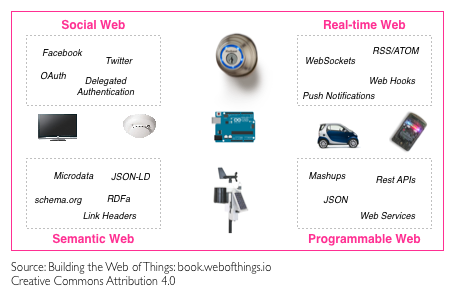
\includegraphics[scale=0.7]{iotweb.png}
  \caption{Il Web of Things è la capacità di utilizzare gli standard web
moderni direttamente su dispositivi embedded.}
  \label{fig:iotweb}
\end{figure}

Questo rende il Web il substrato ideale per la creazione di un'architettura
``universale'' e di Application Programming Interface (API) con cui gli
oggetti possono interagire.

In pratica, questo significa che l'utente può iniziare a interagire con gli
oggetti via Web.

I dati real-time raccolti da sensori distribuiti possono essere facilmente
recuperati, elaborati e visualizzati in pagine Web utilizzando HTML, CSS e
JavaScript.

\begin{figure}[H]
  \centering
  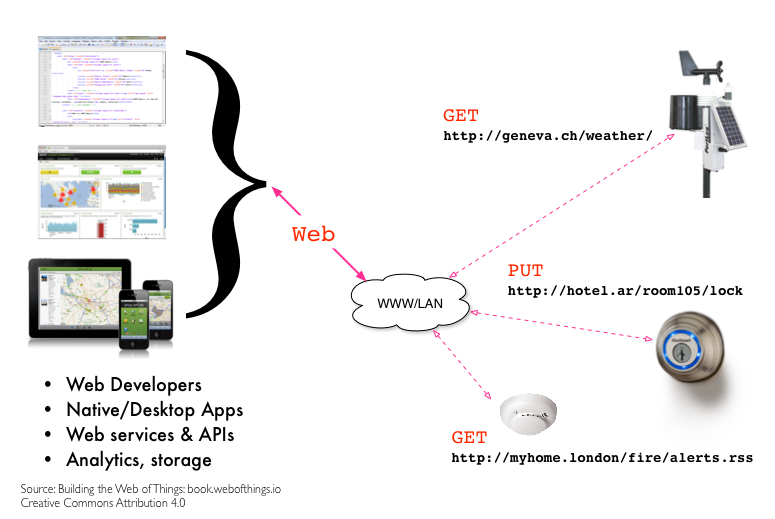
\includegraphics[scale=0.5]{iotrest.png}
  \caption{Un URL per ogni oggetto e un'API RESTful.
Il Web of Things consente agli sviluppatori e alle applicazioni di scambiare
dati con qualsiasi dispositivo che utilizza le richieste HTTP / WebSockets
standard, indipendentemente dal modo in cui il dispositivo è collegato.}
  \label{fig:iotrest}
\end{figure}

\textbf{MA} anche se i protocolli Web sono disponibili e utilizzabili per i
dispositivi IoT, possono essere troppo pesanti per alcune applicazioni di IoT.
Diamo un'occhiata ad altri protocolli.

\subsection{Non tutti usano HTTP}

\textbf{MQTT}\\

MQ Telemetry Transport (MQTT) è un protocollo open source per devices con
vincoli di banda e reti con alta latenza.

Ha un trasporto di messaggistica publish/subscribe che è estremamente leggero.

MQTT è efficiente in quanto a consumi di banda e data agnostic.
Aiuta a ridurre al minimo i requisiti di risorse per un dispositivo IoT,
pur tentando di garantire l'affidabilità del trasporto.

\textbf{Proprietà:}

\begin{itemize}
  \item modello client/server
  \item i clients si iscrivono ai canali in base a dei ``topic di interesse''
  \item i canali per i topic sono gerarchici (es. room2BC/heating)
  \item 3 livelli QoS: ``Fire and forget'',  ``delivered at least once'' e
 ``delivered exactly once''.
  \item autenticazione basata su username/password
  \item TCP over SSL/TLS
\end{itemize}

\textbf{CoAP}\\

Il Constrained Application Protocol (CoAP) è stato progettato per essere
utilizzato su reti vincolate e a basso consumo. CoAP è un protocollo RESTful.
È semanticamente allineato con HTTP e ha persino un mapping uno-a-uno da e
verso HTTP.\\

\textbf{Proprietà:}

\begin{itemize}
  \item i pacchetti sono molto più piccoli rispetto a HTTP TCP.
  \item (simpler and faster to parse with small memory footprint) ?
  \item In UDP, interagisce con HTTP e il web RESTful attraverso semplici
proxies
  \item modello client/server, in cui i clients possono chiamare GET, PUT,
POST and DELETE per ottenere/modificare/inserire/cancellare risorse.
  \item I dispositivi CoAP in grado di supportare DTLS supportano RSA e AES o
ECC e AES
\end{itemize}

\begin{figure}[H]
  \centering
  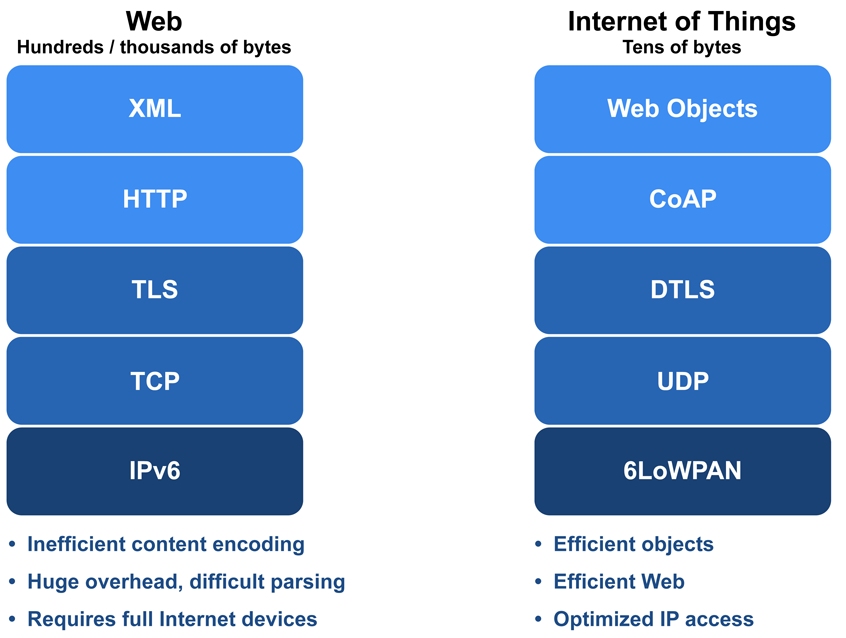
\includegraphics[scale=0.4]{protocol_comparison.png}
  \caption{Sulla sinistra, lo stack di protocollo per applicazioni Web può
facilmente produrre un overhead di dati di centinaia o migliaia di byte.
A destra invece, i protocolli IoT sono ottimizzati per dispositivi e reti
vincolati, e producono un overhead di dati molto più piccolo (decine di
byte).}
  \label{fig:protocol_comparison}
\end{figure}

\subsection{Integration Patterns}

\textbf{Comunicazione diretta}

Nel caso più semplice, una Web Thing è semplicemente una API alla quale i
clients inviano richieste.

Il Client e la Web Thing possono essere sulla stessa rete o meno.

\begin{figure}[H]
  \centering
  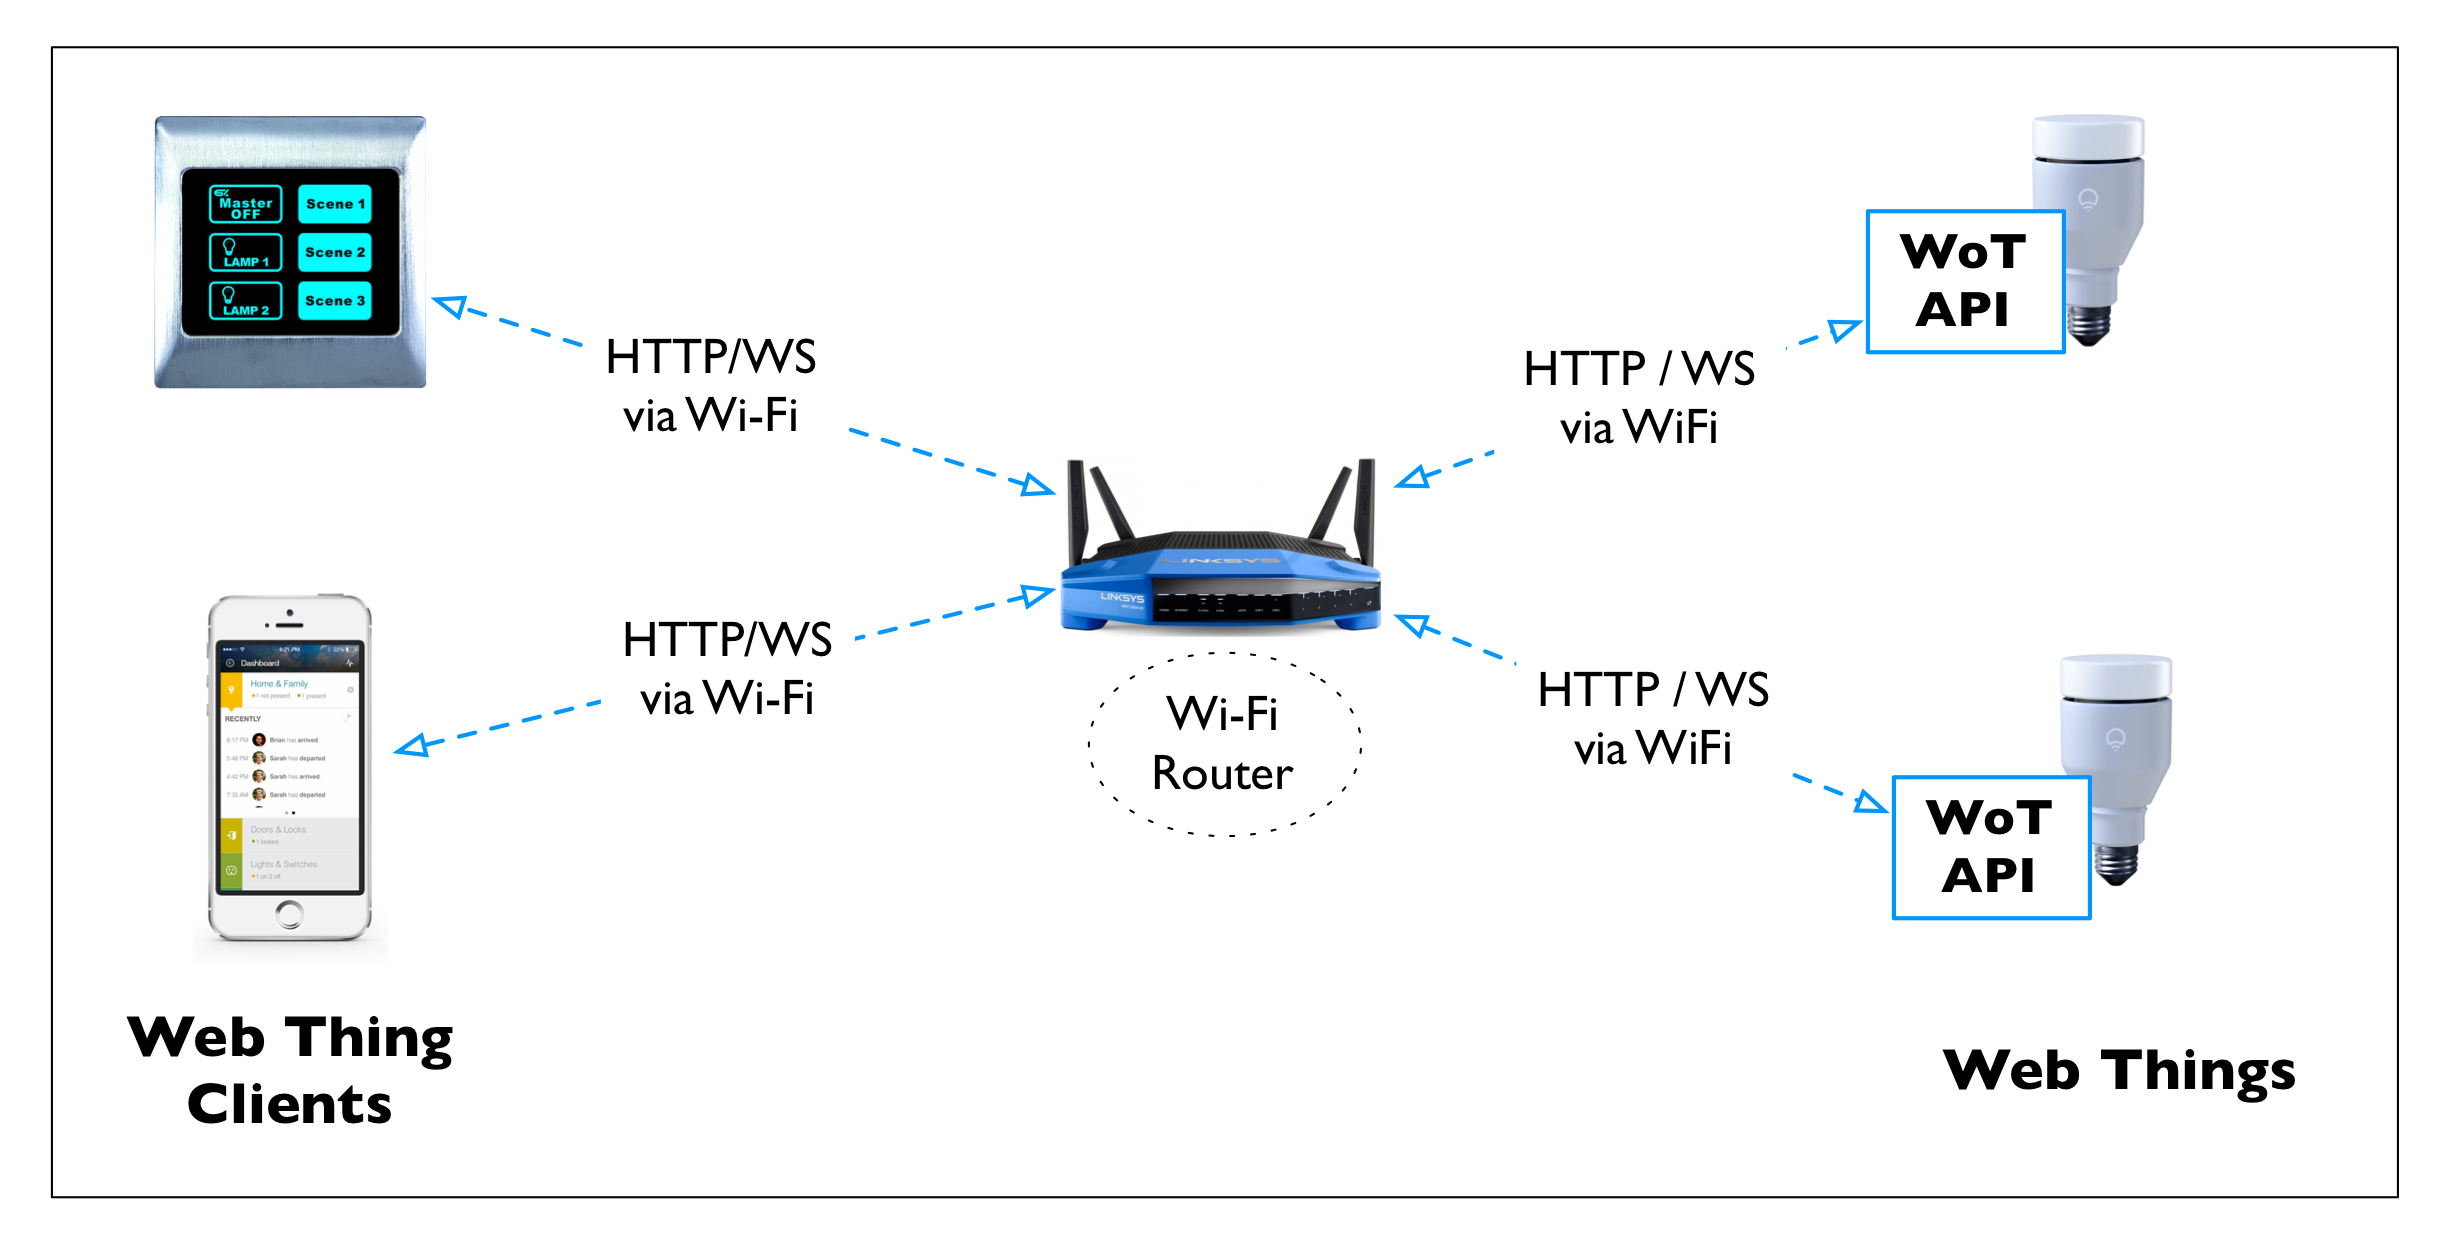
\includegraphics[scale=0.5]{direct_communication.png}
  \caption{Comunicazione diretta tra un client e una web thing}
  \label{fig:direct_communication}
\end{figure}

\textbf{Gateway}

La connettività/comunicazione basata su gateway viene utilizzata quando un
oggetto non può offrire direttamente un'API Web.

In questo caso una Web Thing intermedia - il gateway - espone un'API Web
per conto dell'oggetto.

La Web Thing quindi funge da proxy per l'oggetto (o da gateway a seconda della
complessità della traduzione).

\begin{figure}[H]
  \centering
  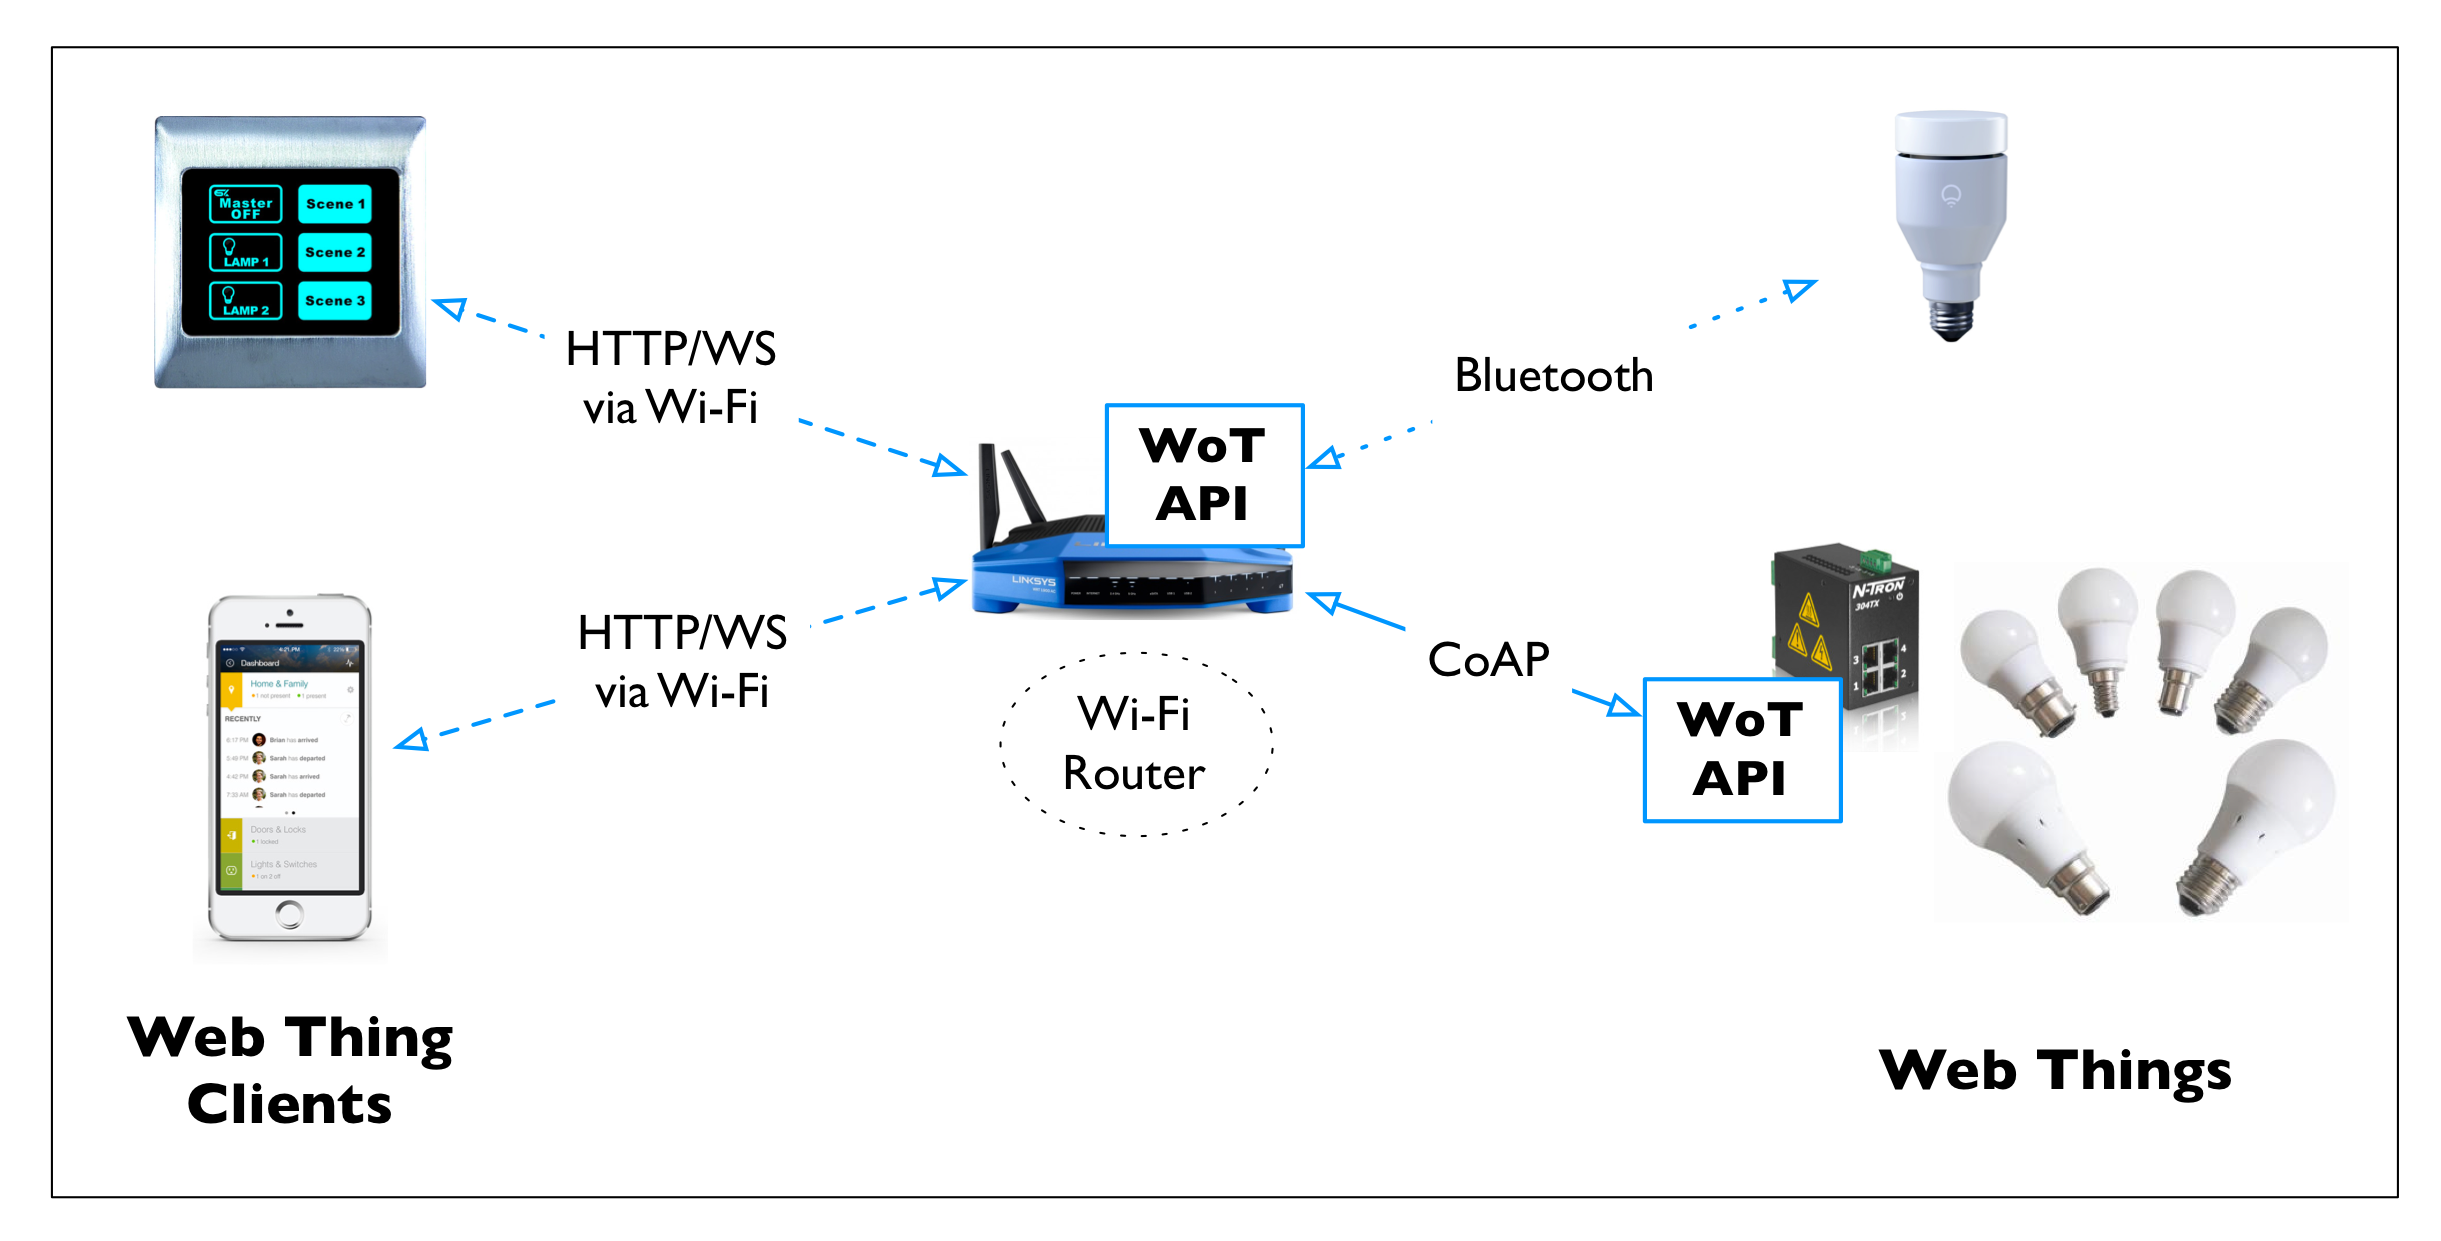
\includegraphics[scale=0.5]{gateway.png}
  \caption{Connettività basata su gateway tra un client e una web thing}
  \label{fig:gateway}
\end{figure}

\textbf{Cloud}

Il terzo caso è simile al precedente ma questa volta il gateway è un servizio
cloud.

\begin{figure}[H]
  \centering
  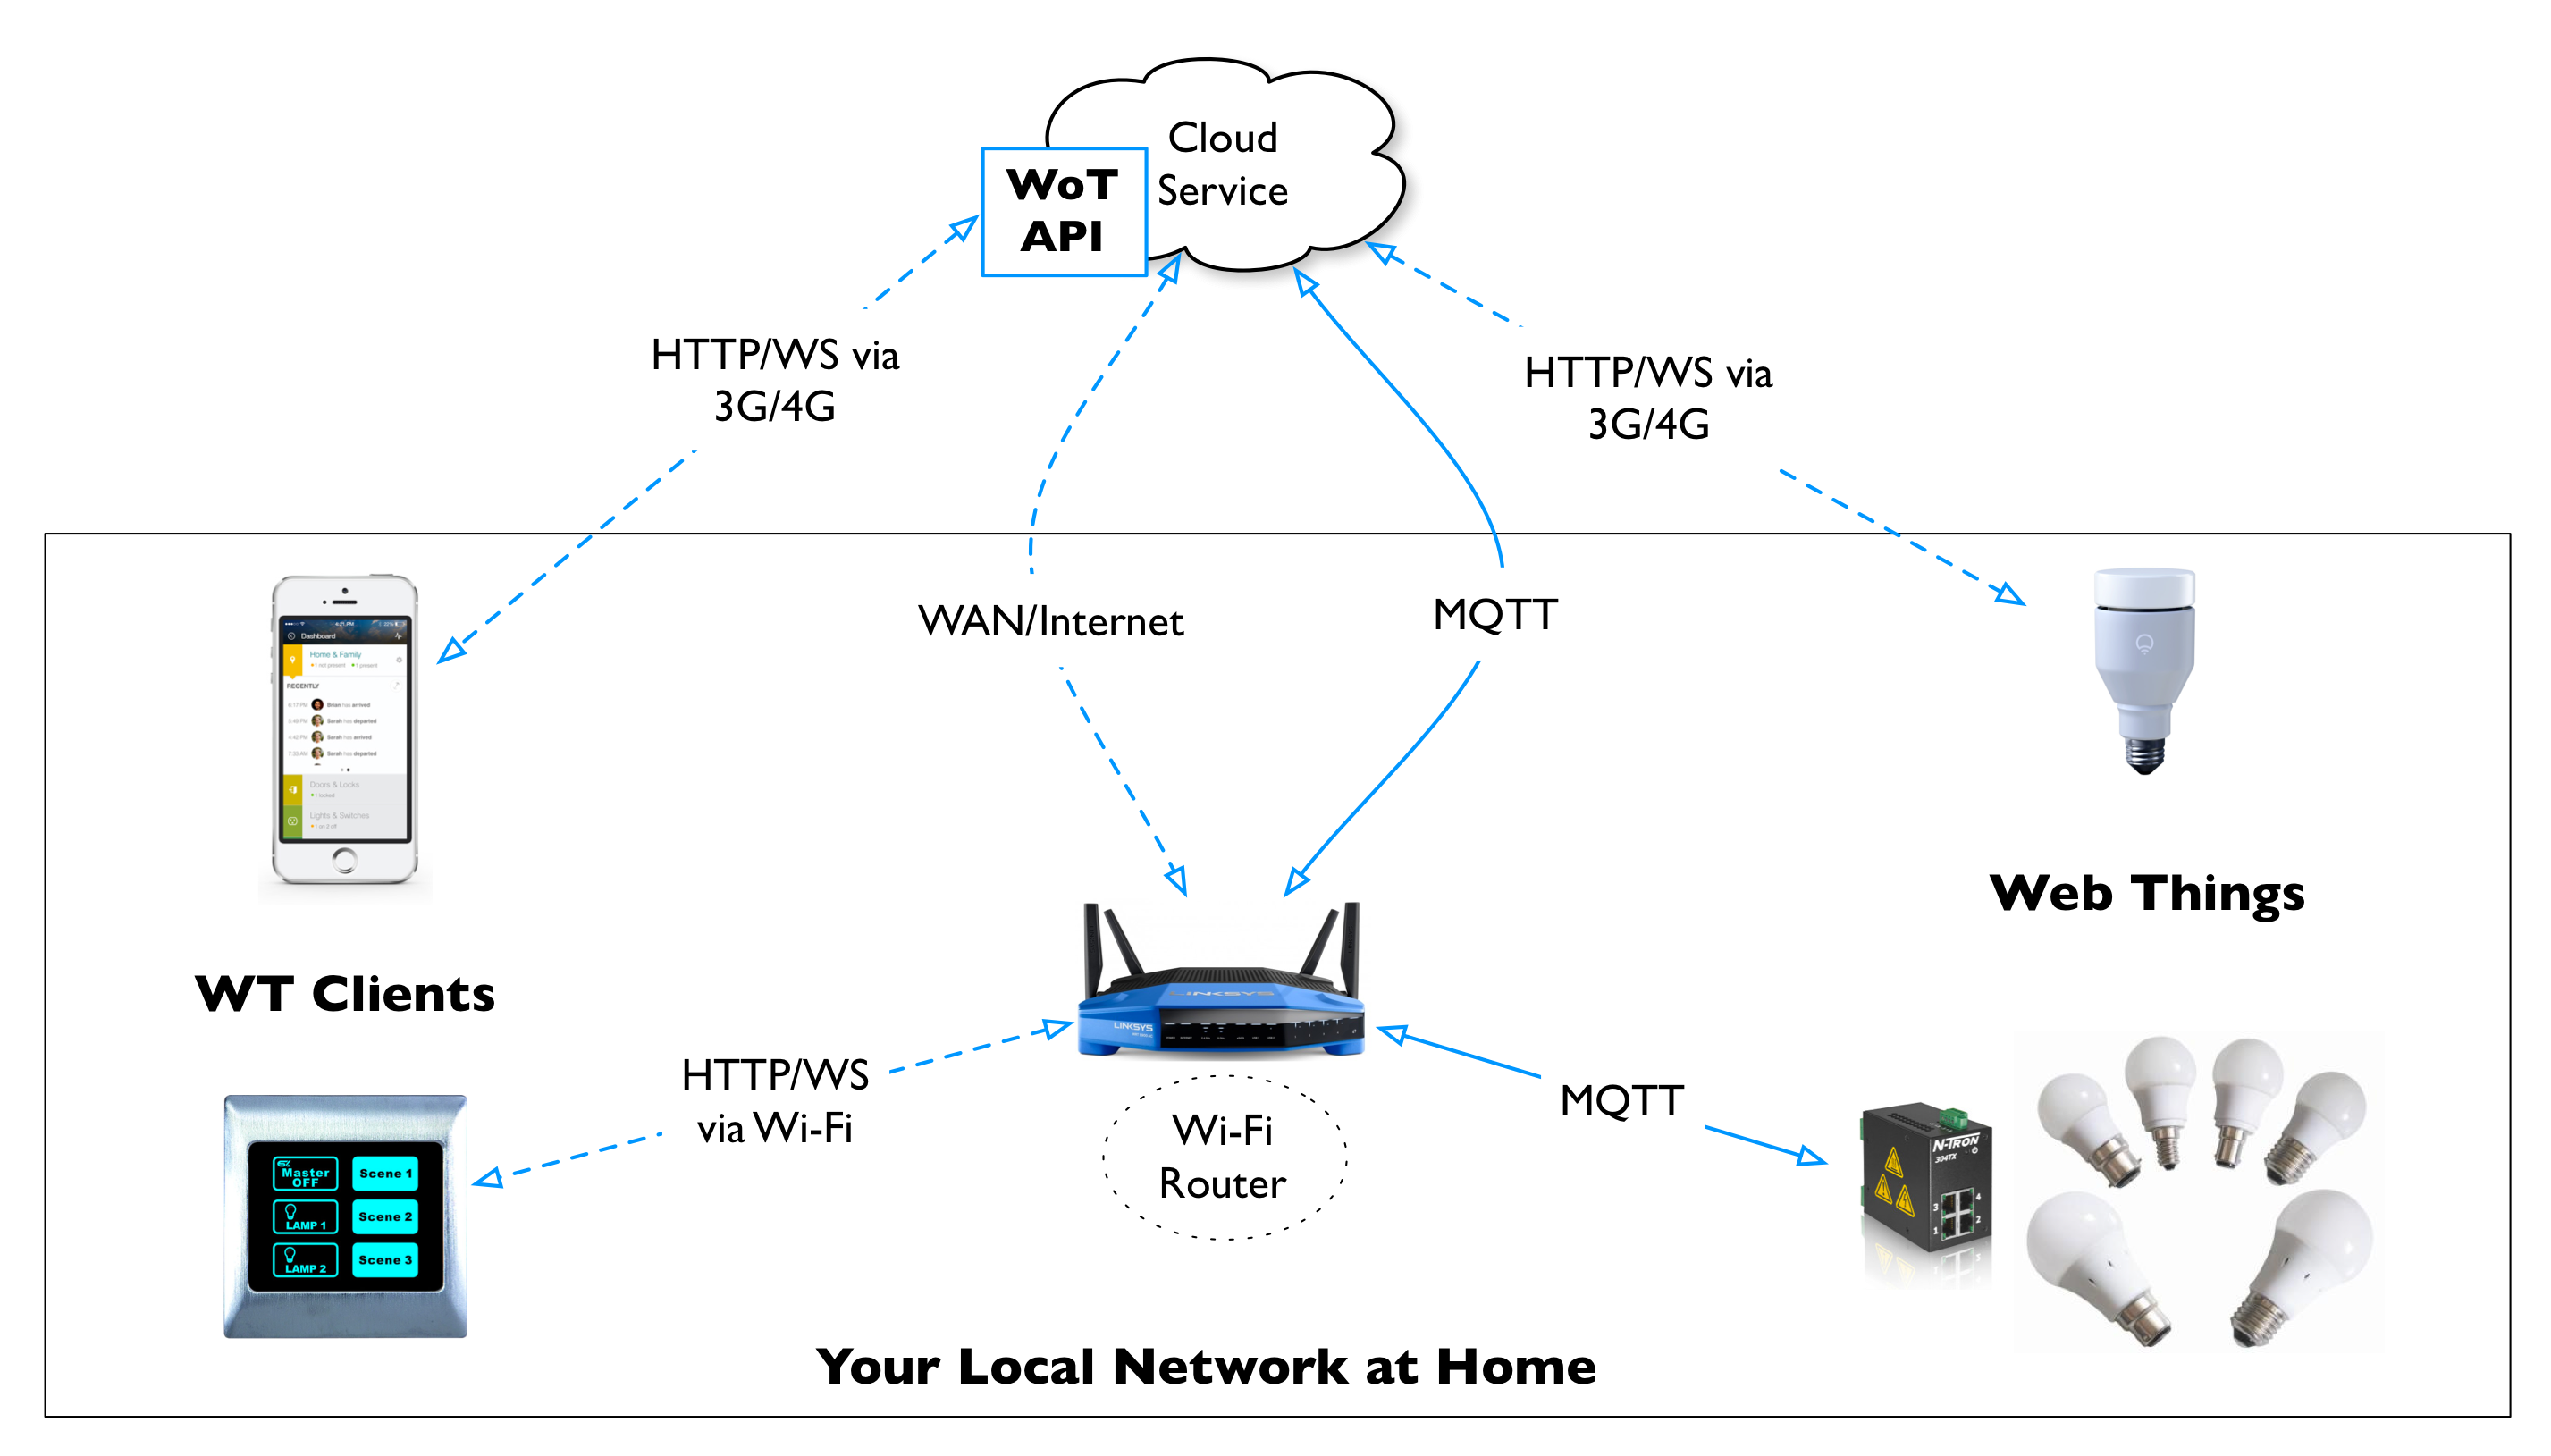
\includegraphics[scale=0.5]{cloud.png}
  \caption{Connettività basata su cloud tra un client e una web thing}
  \label{fig:cloud}
\end{figure}

\subsection{Web of Things Architecture}

Anche se ci sono dei tentativi in corso per standardizzarlo, il Web of Things
è per il momento un insieme di \textit{best practices} che possono essere
classificate in 4 livelli.

L'architettura del Web of Things propone quattro livelli principali che vengono
utilizzati come framework per classificare i diversi patterns e protocolli
coinvolti.

\begin{figure}[H]
  \centering
  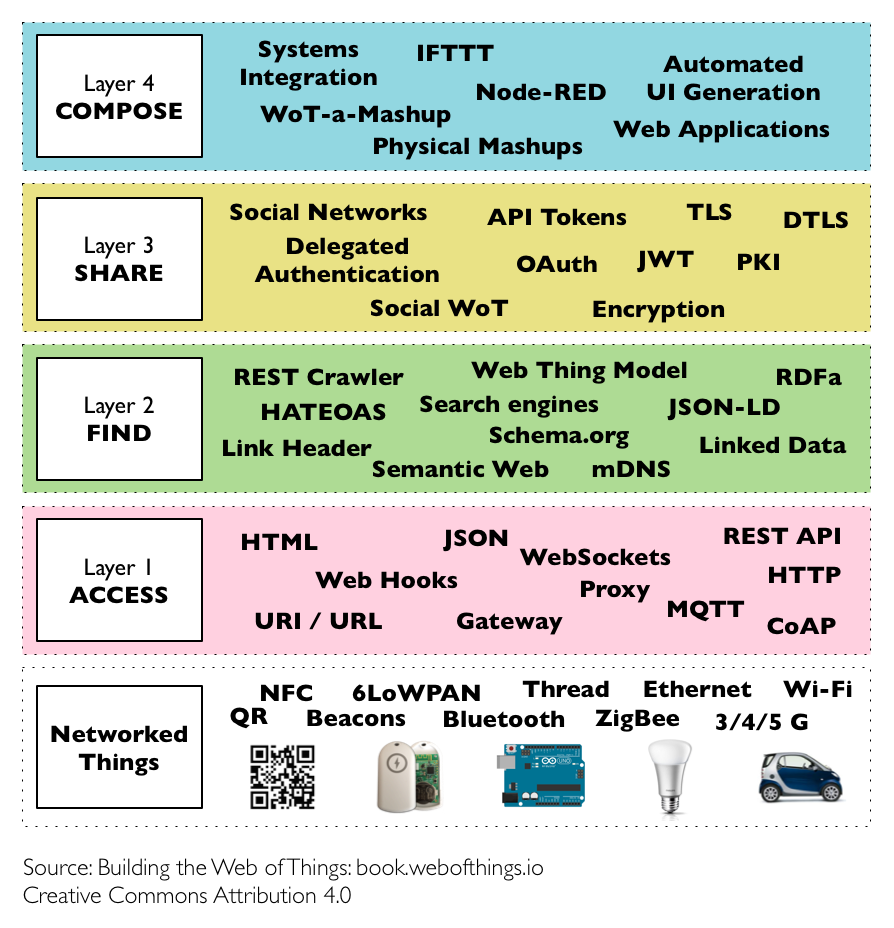
\includegraphics[scale=0.5]{wotarchitecture.png}
  \caption{Architettura del Web of Things}
  \label{fig:wotarchitecture}
\end{figure}

\textbf{Accessibility layer - Accessibilità}\\

Questo livello riguarda l'accesso degli oggetti ad
Internet e si assicura che espongano i propri servizi tramite API Web
(già discusso nelle sezioni precedenti di questo capitolo). \\

\textbf{Findability layer - Localizzazione}\\

Rendere oggetti accessibili tramite un'applicazione HTTP e WebSocket è ottimo,
ma ciò non implica che poi le applicazioni sappiano davvero ``capire''
cosa fanno gli oggetti, quali dati o servizi offrono, ecc \dots.

Qui entra in gioco il secondo livello - Localizzazione.
Questo livello assicura che un oggetto non solo possa essere facilmente
utilizzato da altri clients HTTP, ma possa essere anche individuabile e
utilizzabile automaticamente da altri applicazioni di tipo WoT.

L'approccio qui è quello di riutilizzare gli standard del web semantico per
descrivere gli oggetti e i loro servizi.

Ciò consente di cercare gli oggetti attraverso i motori di ricerca e di
generare interfacce o strumenti utente per interagire con essi. \\

\textbf{Sharing layer - Condivisione}\\

L'IoT fiorirà solo se gli oggetti avranno un modo di
condividere dati in modo sicuro tra più servizi.

Di ciò si occupa il livello di condivisione, che specifica come i dati
generati dagli oggetti possano essere condivisi in modo efficiente e sicuro
nella rete.

A questo livello, un altro gruppo di protocolli Web aiuta.
Ad esempio, TLS, il protocollo che rende sicure le transazioni sul Web o
meccanismi di autenticazione come OAuth, che possono essere integrati
alle API degli oggetti.

Si possono usare i vari social networks per condividere oggetti e risorse
e creare così un Social Web of Things.\\

\textbf{Composition layer - Composizione}\\

Una volta che gli oggetti sono sul Web (livello 1) dove possono
essere trovati dagli esseri umani e dalle macchine (livello 2) e le loro
risorse possono essere condivise in modo sicuro con gli altri (livello 3),
è tempo di guardare come costruire su larga scala applicazioni significative
per il Web of Things.

In altre parole, dobbiamo capire come integrare dati e servizi da oggetti
eterogenei in un immenso ecosistema di strumenti Web.
Gli strumenti Web nell'ambito del livello di composizione variano da toolkit
web - ad esempio, JavaScript SDK - a dashboard con widget programmabili e,
infine, gli strumenti fisici di mashup come Node-RED (mostrato di seguito).

\begin{figure}[H]
  \centering
  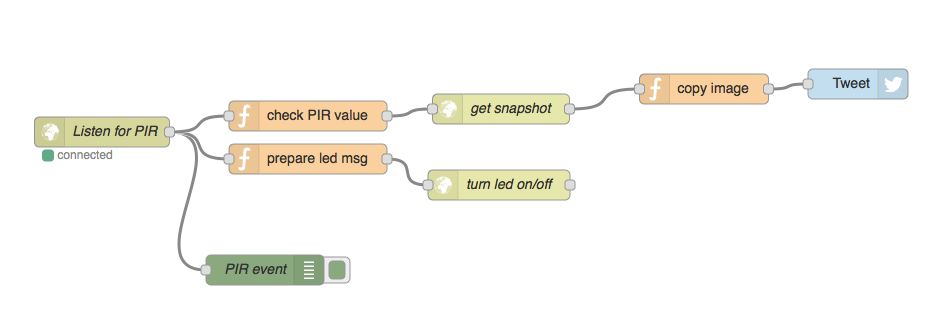
\includegraphics[scale=0.4]{nodered.png}
  \caption{Mashup fisico con Node-RED;
Controllo automatico di un sistema di riscaldamento;}
  \label{fig:nodered}
\end{figure}

\subsubsection{Conclusione}

Web of Things è un protocollo di applicazioni ad alto livello progettato per
massimizzare l'interoperabilità nello IoT.

Le tecnologie Web sono ampiamente diffuse e offrono tutta la flessibilità e le
caratteristiche necessarie per le future applicazioni IoT. \\

\textbf{Fonti:}\\

Un mix di:

\begin{itemize}
  \item slides del corso
  \item \url{http://webofthings.org/2016/01/23/wot-vs-iot-12/}
  \item \url{http://webofthings.org/2017/04/08/what-is-the-web-of-things/}
  \item \url{https://www.micrium.com/iot/internet-protocols/}
  \item \url{https://www.w3.org/blog/wotig/}
\end{itemize}
